\documentclass[10pt,a4paper]{report}
\usepackage[utf8]{inputenc}
\usepackage{amsmath}
\usepackage{amsfonts}
\usepackage{amssymb}
\usepackage{float}
\usepackage{graphicx}
\graphicspath{{./images/}}
\usepackage{mathtools}
\DeclarePairedDelimiter\abs{\lvert}{\rvert}
\usepackage[left=3.00cm, right=3.00cm, top=3.00cm, bottom=3.00cm]{geometry}
\author{Del Prete Giovanni, Ghilardi Nicola, Polver Marco}

\title{BookSales UniBG: iterazione 2}
	

\begin{document}
\maketitle
	\tableofcontents
	\section{Algoritmo: il clustering}
	Il clustering è un algoritmo di apprendimento non supervisionato (machine learning) che ha l'obiettivo di ricercare gruppi di oggetti tali che  
	gli oggetti appartenenti a un gruppo siano “simili” tra loro e differenti dagli oggetti negli altri gruppi. Dunque, in statistica, è una tecnica di 
        analisi multivariata dei dati volta al raggruppamento di elementi omogenei in un insieme di dati.\\
        Oggi le tecniche di clustering sono diffuse in diversi campi applicativi, tra i quali: il marketing, l'analisi del territorio, le assicurazioni  gli studi sismici e l'image processing.  Uno degli usi più comuni che viene fatto dei cluster, in ambito economico, 
        è proprio la segmentazione di mercato, che può essere riferita a consumatori o a categorie di prodotti con lo scopo di valutare le caratteristiche e i comportamenti dei consumatori, personalizzando l’offerta
        e incrementando dunque la quantità di prodotti venduti.
        \begin{figure}[H]
		\centering
		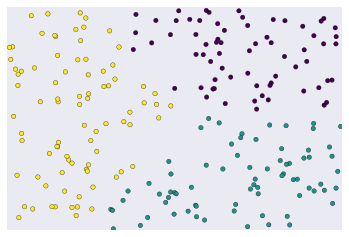
\includegraphics[scale=0.9]{Cluster.png}
		\caption{Cluster}
		\end{figure}
		\newpage

        \subsection{K-means clustering}
        		Il k-means clustering è l'algoritmo di clustering più utilizzato sia in ambito accademico che in ambito industriale e funziona nel seguente modo.
        		\begin{enumerate}
        		\item Scegliere il numero di k clusters in cui raggruppare il dataset.
        		\item Selezionare casualmente k centroidi iniziali (con centroide si intende il centro geometrico di ogni cluster).
        		\item Calcolare la distanza tra ogni centroide e tutte le osservazioni.
        		\item Assegnare ognuna delle osservazione al cluster rappresentato dal centroide più vicino.
        		\item Ricalcolare la posizione dei centroidi come la posizione media delle osservazioni appartenenti al cluster che il centroide rappresenta.
        		\item Ripetere dal punto 3, finchè nessuna osservazione cambierà più il proprio cluster di appartenenza.
        		\end{enumerate}
		\textbf{Problema}: come scegliere a priori il numero di clusters k?\\
		La soluzione a questo problema sta nel testare in modo iterativo più valori di k e confrontarli. 
		Per valutare il risultato viene analizzata la funzione di costo:
		\[
		J(k)=\frac{1}{k}
		\sum_{i=1}^k
		\frac{1}{n}
		\sum_{j=1}^n
		\abs{p\textsubscript{j}-c\textsubscript{i}}
		\]
		Tale funzione di costo è la media delle distanze medie delle osservazioni dal centroide del proprio cluster. E' facile notare che aumentando il numero di
		cluster diminuirà, di conseguenza, la media delle distanze delle osservazioni dai centroidi; dunque la funzione di costo è decrescente.\\
		L'\textit{elbow method} è un metodo ''grafico'' che consente di determinare il numero di cluster ideale valutando la pendenza della funzione di costo.
		Come si evince dalla figura 4, il valore ottimo di k è prossimo al punto dove la funzione di costo inizia a decrescere più lentamente, dunque in questo caso d'esempio,
		vale 3.
		\begin{figure}[H]
		\centering
		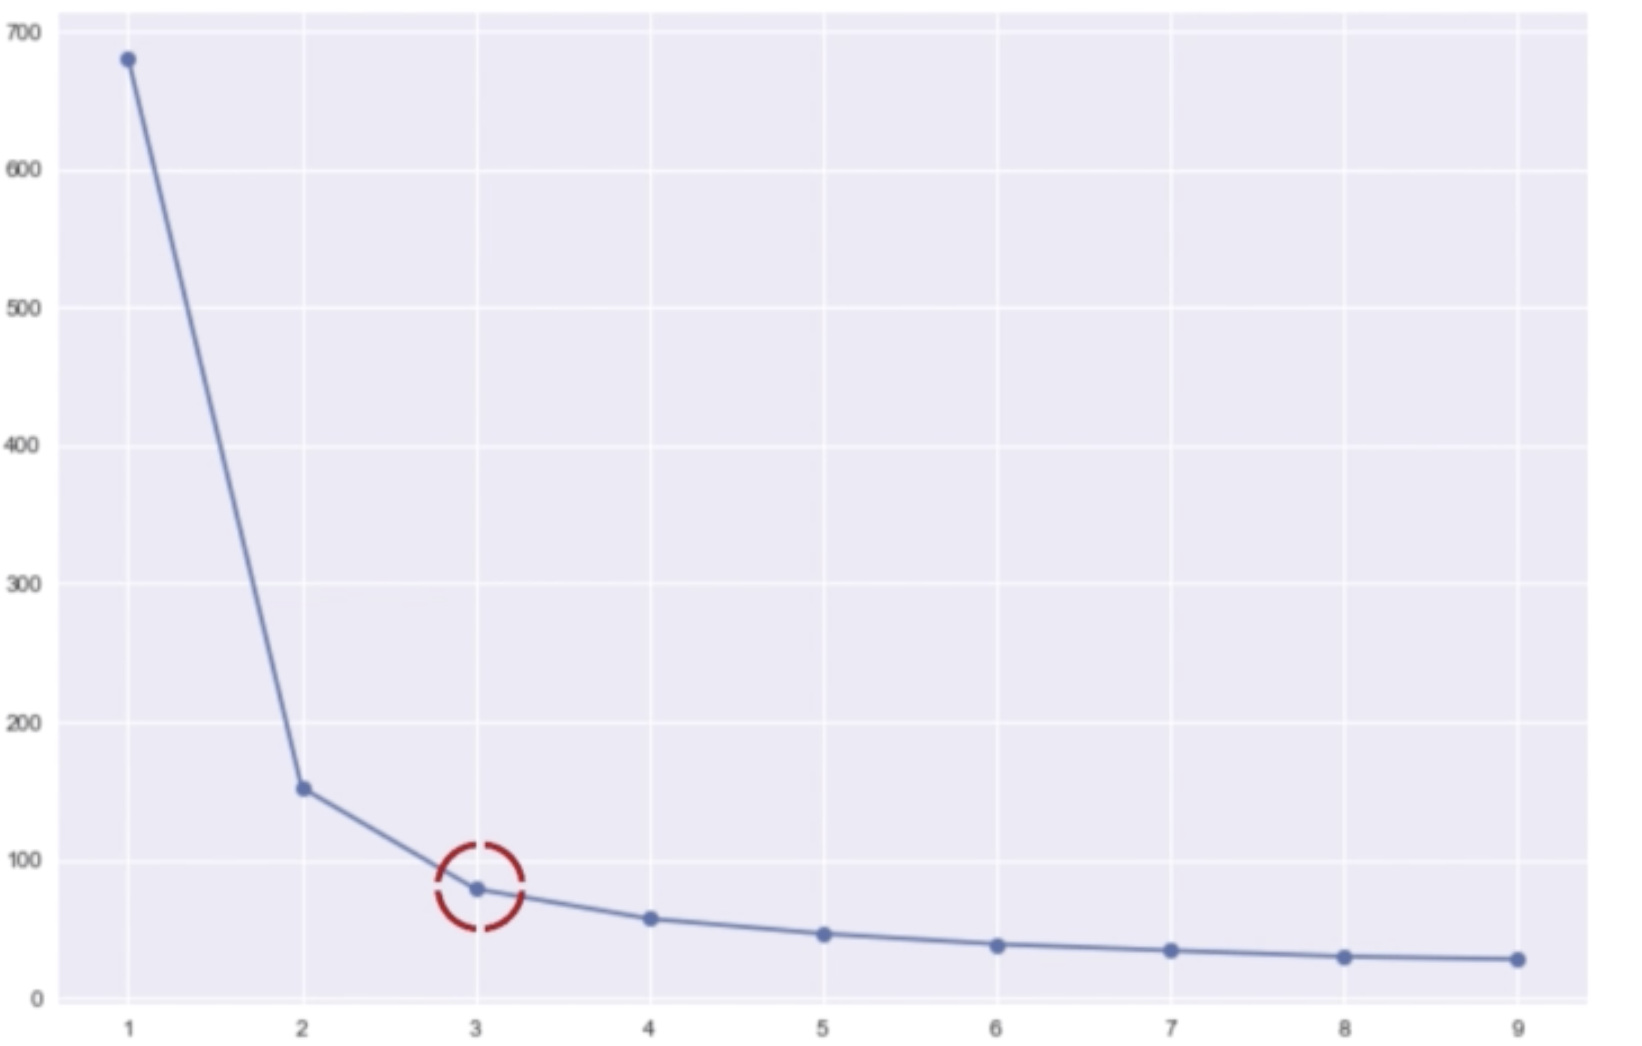
\includegraphics[scale=0.5]{elbow_method.png}
		\caption{Elbow method}
		\end{figure}
	\subsection{Il clustering in BookSales Unibg}
	L'algoritmo di k-means clustering è stato utilizzato in BookSales Unibg con l'obiettivo di suddividere in cluster gli utenti sulle basi dei loro interessi.\\
	L'algoritmo assegna ad ogni studente un cluster di appartenenza basandosi sui titoli presenti nella sua Wish List e Interesting Title. Ogni libro 
	presente in BookSales Unibg appartiene ad una categoria: le features di ogni studente sono il numero di libri che interessano allo studente 
	appartenenti ad ogni categoria.
	Le categorie in cui sono stati suddivisi i libri sono:
	\begin{itemize}
		\item Fisica
		\item Matematica
		\item Informatica
		\item Meccanica
		\item Elettronica
		\item Economia
		\item Automazione
	\end{itemize}
	L'algoritmo di clustering viene eseguito ogni volta che uno studente, dopo il login, entra nella pagina Suggested Adds, solo se è passata almeno un'ora 
	dall'ultima esecuzione. Nel caso in cui sia passata meno di un'ora dall'ultima esecuzione, vengono utilizzati i risultati di tale esecuzione.
	Dopo i risultati del clustering, ogni studente vedrà nella pagina Suggested Adds i titoli in linea con i propri interessi.\\
	Dato il numero elevato di features e di cluster non è possibile visualizzare graficamente i risultati di un'esecuzione dell'algoritmo.
	
	
		


\end{document}
	